%In this section we provide details of the three datasets that we evaluate in this paper, as well as the methodology used.
%\subsection{Dataset description}


%\subsubsection{Twitter example (Detection of natural disasters)}
In this section, we first describe the dataset used for our experiments, then we describe the baselines we used for comparison.
\subsection{Dataset description}
The scenario we have chosen to evaluate our algorithms is related to the detection of natural disasters discussed in a collection of tweets.  We started with a corpus of approximately 1 billion tweets crawled from the Twitter streaming API during 2013 and 2014 with the following restrictions:
%the Twitter data described in~\cite{Iman2017}:
%, which was curated by four students as follows: 
(1) the dataset was restricted to users located within the US, (2) non-English tweets were filtered out, (3) only the tweets related to 12 natural disasters were kept -- tweets related to other natural disasters were removed. These natural disasters are temporally, and geographically disjoint -- a storm, a hurricane,  a drought, two floods, two earthquakes, two tornadoes,  and three blizzards. Finally, (4) false positive tweets (i.e., tweets mentioning natural disasters specific-keywords but are not related to a particular natural disaster) from the dataset were intentionally included, e.g., \textit{\textquotedblleft I'm flooded with questions from followers\textquotedblright{}}. The final dataset contains 39,486 tweets with 5,075 marked as relevant tweets (in this context, a relevant tweet is a tweet related to a natural disaster).

\subsection{Baselines description}
We used the following two baselines for comparison:

\subfour{Optimal solution:} To benchmark the performance of the greedy algorithms we proposed on moderately sized datasets, we use an 
exact Mixed Integer Linear Progamming (MILP) optimization-based formulation to maximize EF1. In brief, the formulation of EF1 in Equation \ref{eq:EF1} can be transformed into a fractional MILP formulation with constraints corresponding to each of the cluster attribute selection criteria (space, time, and content).  The parameters of these constraints are then chosen to optimize the EF1 objective.

Because there are no direct solvers for fractional MILPs, we can transform the problem into a pure MILP formulation for which we have efficient and optimal solvers using the Charnes-Cooper method \cite{Charnes1962} and Glover linearization method \cite{Glover1975} with big-M constraints.  
%Lastly, we add three constraints to the optimization to select elements through three clustering parameters, i.e., time, position and keywords. %We refer the reader to [ADD ANONYMOUS CITATION?] for more details o this method.




 
\subfour{K-Means clustering:} In addition, we also propose to use X-Means \cite{Pelleg2000} as a baseline method for clustering. X-Means is a simple extension of K-Means~\cite{kmeans_original} which tries to  automatically determine the number of clusters. Starting with only one cluster, the X-Means wrapper applies after each run of K-Means, making local decisions about which subset of the current centroids should split themselves in order to better fit the data.  In order to provide X-means with spatial, temporal, and content coherence, the distance metric we have used for X-Means is a linear combination of the following: (i) the Euclidean distance of time, (ii) the Euclidean distance of location, and (iii) the cosine distance of the textual content. This distance metric is formally defined as follows:
\begin{equation}
\begin{array}{ll}
d(i,j)= & \alpha\times\textrm{[time distance]} +\\
& \beta\times\textrm{[location distance]}+\\
 & \gamma\times\textrm{[text cosine distance]}
\end{array}
\end{equation}
\noindent where $\alpha$, $\beta$, and $\gamma$ are weights that sum to 1, set all to 1 in the off-line evaluation and set respectively to 0.1, 0.8,  and 0.1 in the user study -- values manually tuned in extensive pilot user trials to maximize cluster quality.  Once clusters are extracted by X-means, we use the EF1 metric to extract the top clusters as required by our interface.

%We assume having an agent monitoring tweets, a topical tweets classifier (e.g., \cite{Iman2017}), and a display showing the locations of the tweets (See Figure \ref{Fig:TwitterData}).  We used the  2.5 TB of Twitter data described in  \cite{Iman2017}, for which we restricted our analysis to the 9M tweets of January 2014.





%\begin{figure}[t]
%\begin{centering}
%\subfigure[Twitter Networks.]{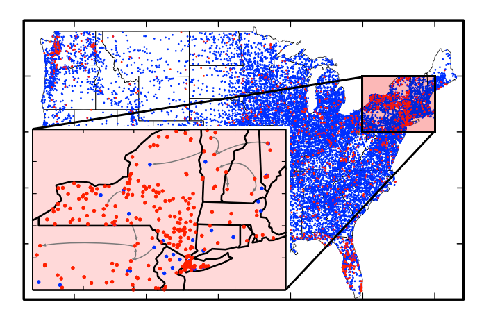
\includegraphics[width=2.8cm]{imgs/twitter_example_3}\label{Fig:TwitterData}}\subfigure[Enron Networks.]{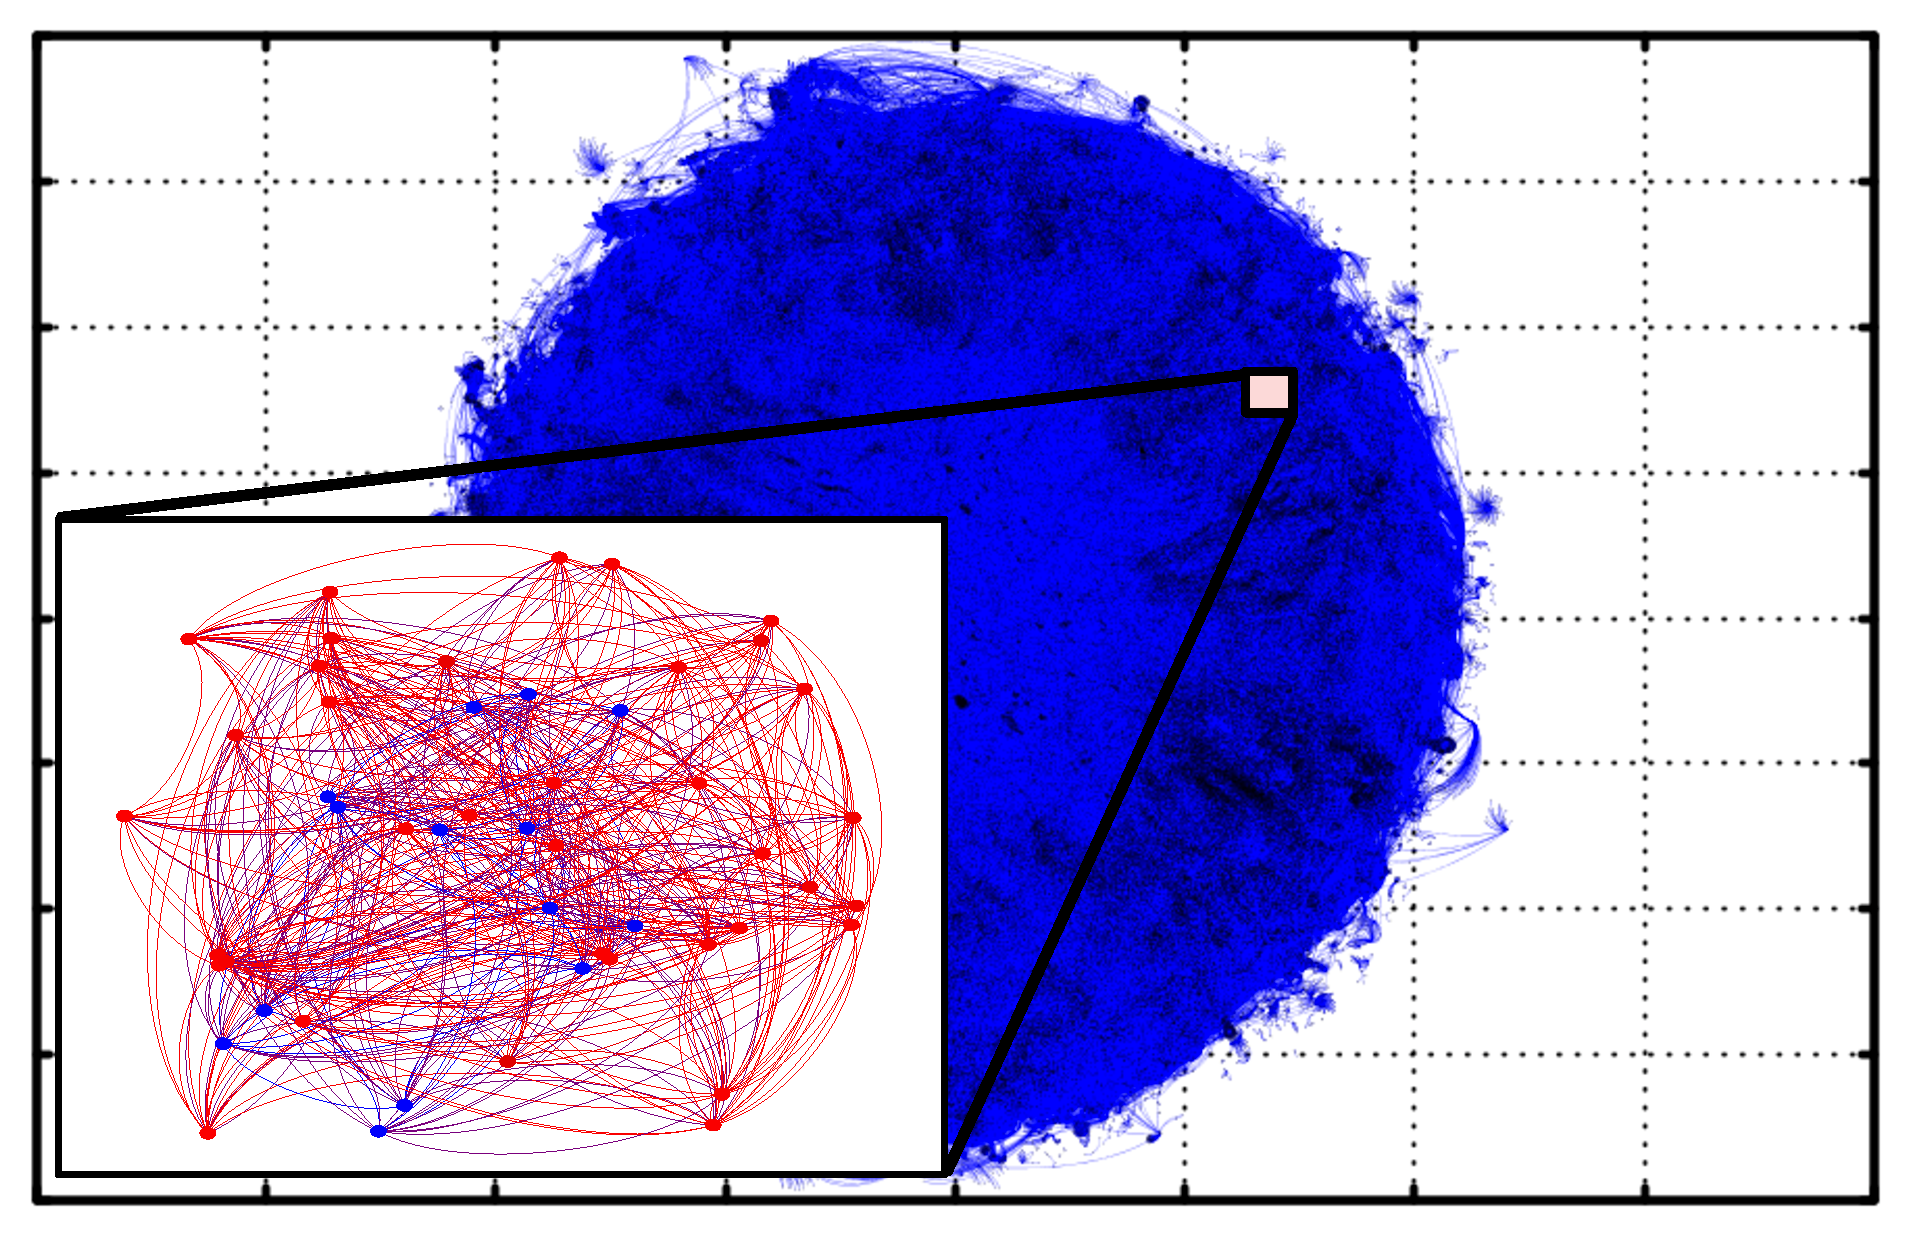
\includegraphics[width=2.8cm]{imgs/enron_net_4}\label{Fig:EnronData}}\subfigure[Reddit Networks.]{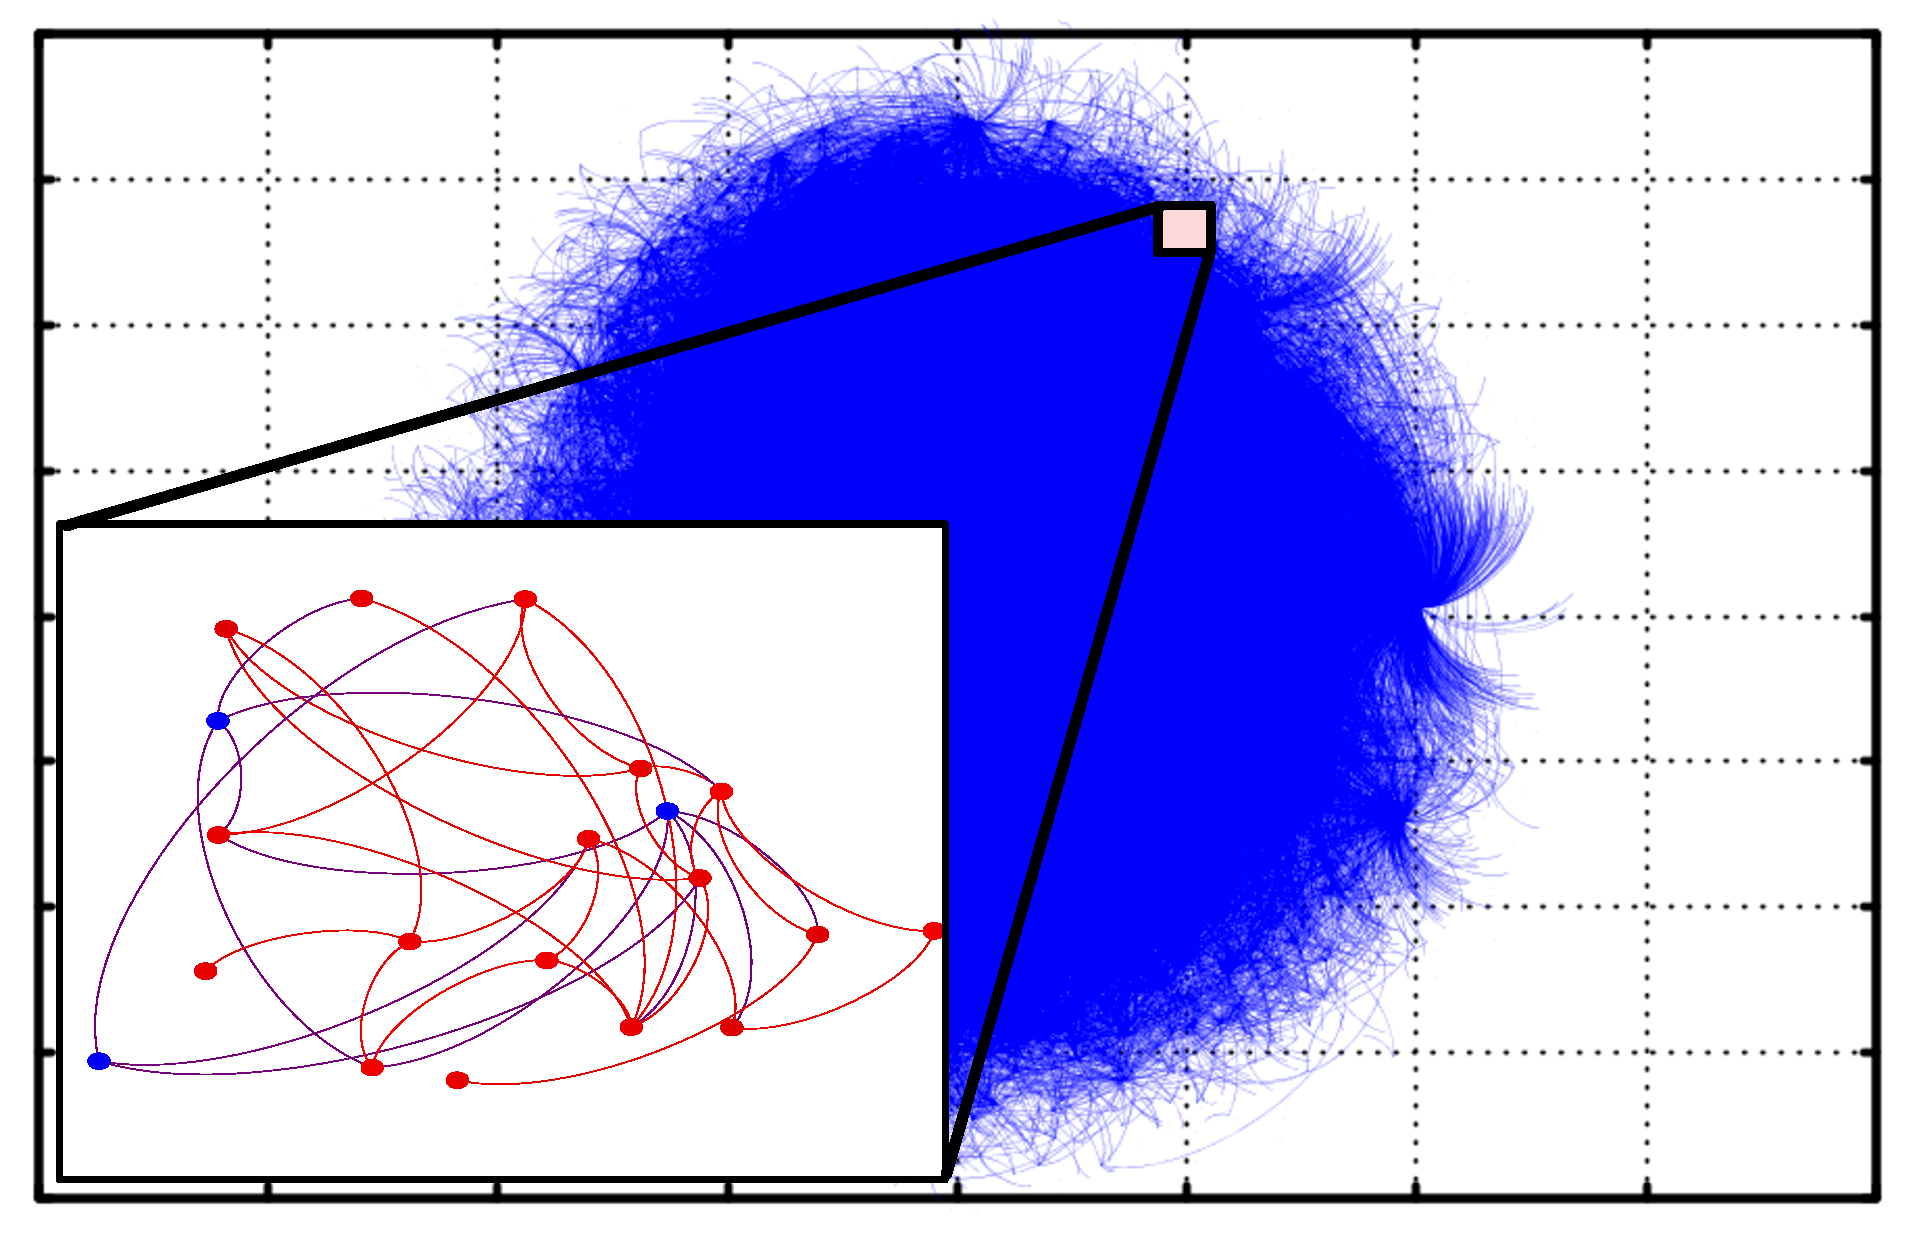
\includegraphics[width=2.8cm]{imgs/srforum3}\label{Fig:RedditData}}
%\par\end{centering}
%\caption{Layouts used for the different datasets.}
%\end{figure}





